\documentclass{beamer}
\usepackage[utf8]{inputenc}
\usepackage[english]{babel}
\usepackage{amsmath}
\usepackage{enumitem}
\usepackage{csquotes}
\usepackage{apacite} 
\usepackage{hyperref}
\usepackage{multimedia}
\definecolor{BlueGreen}{cmyk}{0.85,0,0.33,0}
\definecolor{pink}{rgb}{1,.1,0.6}
\definecolor{orange}{rgb}{1,.5,0}
\definecolor{yellow}{rgb}{1,1,0}
\definecolor{Magenta}{cmyk}{0,1,0,0}
\usepackage{graphics}
\usepackage{amsfonts}
\setbeamercovered{transparent}
\usepackage{array}
\usepackage{amssymb}
\usepackage{graphicx}
\usepackage{amsfonts}
\usepackage{amsmath}
\usepackage{url}
%\usetheme[progressbar=frametitle]{metropolis}
\setbeamertemplate{frame numbering}[fraction]
\useoutertheme{metropolis}
\useinnertheme{metropolis}
\usefonttheme{metropolis}
\usecolortheme{seahorse}
\usepackage{cite}
\setbeamercolor{background canvas}{bg=white}
\setbeamerfont{subsection in toc}{size=\footnotesize}



\title{Modelado del Efecto Mcgurk,un fenónemo de integración multimodal}
\author{Marco Antonio Flores Coronado\\ Tutor: Dr Bruno Lara}
\institute[Laboratorio de Robótica Cognitiva, CInC, UAEM]  {Laboratorio de Robótica Cognitiva, CInC, UAEM \\ 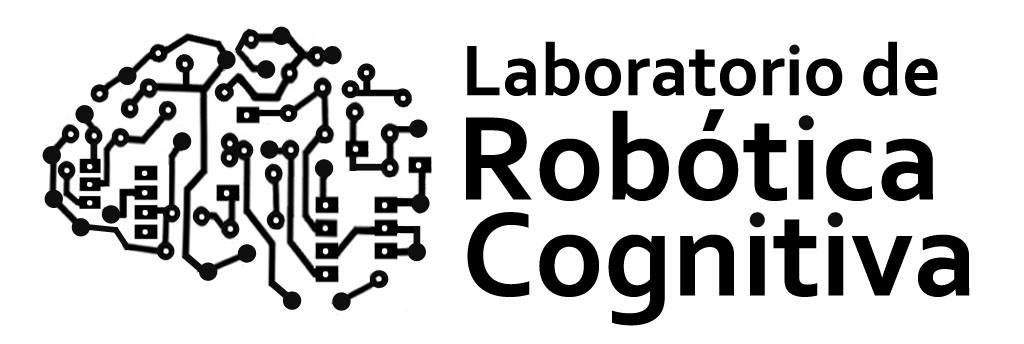
\includegraphics[height=2cm, width=6cm]{images/logo}
\includegraphics[height=1cm, width=3cm]{images/logo_cinc}}
\date{7 de diciembre del 2020}
\begin{document}



\begin{frame}
\frametitle{Marco Antonio Flores Coronado}
\begin{columns}
\column{.3\textwidth}

\includegraphics[width=.7\textwidth]{images/bcbl}
\column{.7\textwidth}
Education
\begin{tiny}
\begin{center}
\textbf{Bachelor in Hispanic Language and Literature}, National Autonomous University of Mexico\\
\textbf{Master in Science} (Cogntive Robotics) Autonomous University of Morelos State\\
\textbf{Predoctoral researcher} Basque Center on Congnition Bran and Language
\end{center}
\end{tiny}
\end{columns}
Research Experience:\\
\begin{flushleft}
\begin{tiny}
\begin{itemize}
\item{\textbf{Signal Processing in Neuroimaging}}(2022-), Basque Center on Congnition Bran and Language
\item{\textbf{Data analyst, MhGAP} (2021)} PAHO
\item{\textbf{Cognitive Robotics Lab} (2019-2022), Center for Science Investigation, UAEM}
\item{\textbf{Cognitive and Language Development Lab} (2018-2022),Psychology School, UNAM}
\item{\textbf{Psycholinguistics Lab} (2016-2022),Psychology School, UNAM}
\end{itemize}
\end{tiny}
Research Interests:\\
\begin{tiny}
\begin{itemize}
\item{Neuroimaging}
\item{Multisensory integration -language-}
\item{Embodied cognition -meaning-}
\item{Language Processing}
\item{Cognitive Robotics}
\item{Language Aquisition -word and meaning- (typical and atypical)}
\item{Lexical networks -semantic and grammar interaction-}

\end{itemize}
\end{tiny}
\end{flushleft}
\end{frame}

\subsection{Research queries}

\begin{frame}
\frametitle{Research queries}
\begin{columns}
\column{.6\textwidth}
\begin{small}
\begin{itemize}
\item<1>{Which is the relevance of multisensory integration in meaning and syntax emergence?}
\item<2>{Which are the neural correlates of affordance based meaning? (i.e., tools Vs. food)}
\item<3>{How do multisensory integration explain non-referential meaning?}
\item<4>{How can we model language development/processing?}
\end{itemize}
\end{small}
\column{.4\textwidth}
\includegraphics<1>[width=\textwidth]{images/multisensory}
\includegraphics<2>[width=\textwidth]{images/covermultisensory}
\includegraphics<2>[width=\textwidth]{images/familiarization}
\includegraphics<3>[width=\textwidth]{images/dead}
\includegraphics<4>[width=\textwidth]{images/architecturePhD.pdf}
\includegraphics<4>[width=\textwidth]{images/robot}
\end{columns}
\begin{center}
\begin{tiny}
\cite{Barsalou2003, Barsalou2018,Kuhnke2020 ,Twomey2020}
\end{tiny}
\end{center}
\end{frame}

\subsection{Modelling of the McGurk effect, a multisensory integration illusion}
\begin{frame}
\frametitle{Modelling of the McGurk effect, a multisensory integration illusion}
\begin{columns}
\column{.3\textwidth}
\begin{center}
\textbf{visual} $ \diagup ga \diagup$\\
\textbf{audition} $ \diagup ba \diagup $ \\
\textbf{perception} $[da]$ \\
\includegraphics<2>[width=.8\textwidth]{images/mc1}
\includegraphics<2>[width=.8\textwidth]{images/mc2}
\includegraphics<3>[width=.8\textwidth]{images/mc3}
\includegraphics<3>[width=.8\textwidth]{images/mc4}
\end{center}
\column{.7\textwidth}
\includegraphics<1-2>[width=1.3\textwidth]{images/mcgurk.png}
\includegraphics<3>[width=1.3\textwidth]{images/mcgurk?}
\end{columns}
\begin{tiny}
\begin{center}
\cite{Mcgurk1976, VanEngen2019, Mitchel2014}
\end{center}
\end{tiny}
\end{frame}


\subsection{Computer Model}
\begin{frame}
\frametitle{Self-Organized Internal Model Architecture (SOIMA)}
\begin{center}
\includegraphics<1>[width=.7\textwidth]{images/soima_mcg.pdf}
\includegraphics<2>[width=.7\textwidth]{images/selectedsoima_mcg.pdf}
\end{center}
\begin{tiny}
\begin{flushleft}
Note. Computer Achitecture. Multysensory integration happens in the Multimodal Representation Map (MMR).
\end{flushleft}
\end{tiny}
\begin{tiny}
\begin{center}
\cite{Escobar-Juarez2016, Morse2017}
\end{center}
\end{tiny}
\end{frame}

\subsection{Feature extraction}

\begin{frame}
\frametitle{Feature extraction/model training}
\begin{columns}
\column{.4\textwidth}
\begin{center}
Vision\\
\begin{tiny}
\textit{Oriented Histograms of Regional Optic Flow}
\end{tiny}
\end{center}
\begin{center}
\movie[autostart,height = 3cm,
  width = 3cm,repeat,
  showcontrols,
  poster]{}{videos/example.avi}
\end{center}
\column{.3\textwidth}
Audition\\
\begin{tiny}
Mel-frequency cepstral coefficients
\end{tiny}
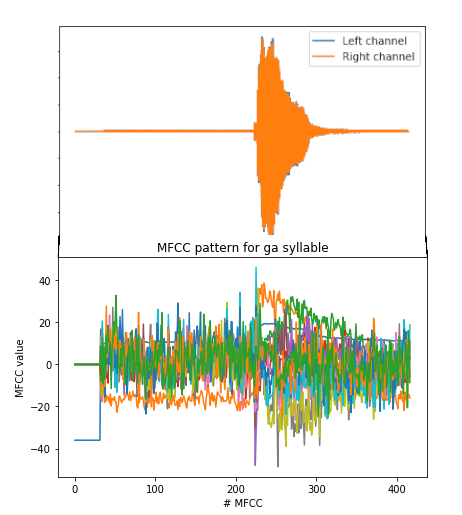
\includegraphics[width=.8\textwidth]{images/MFCC}
\column{.3\textwidth}
Model validation
\begin{tiny}
Psychopy -online-\\ Lipreading experiment \\N$=36$, n$=20$
\end{tiny}
\includegraphics<1>[width=\textwidth]{images/exp}
\includegraphics<2>[width=\textwidth]{images/matriz_confus}
\includegraphics<2>[width=\textwidth]{images/corr_confus}
\end{columns}
\begin{tiny}
\begin{center}
\cite{BasuMallick2015, Viola, Kazemi2014, Liu2016, Gold2011, Hoffman2014}
\end{center}
\end{tiny}
\end{frame}

\subsection{Results}


\begin{frame}
\frametitle{Results}
\begin{columns}
\column{.4\textwidth}
\begin{center}
\begin{tiny}
Congruent and Incongruent stimuli activation
\end{tiny}
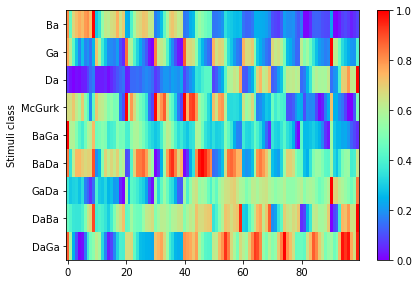
\includegraphics[width=\textwidth]{images/testmatrixmmr}
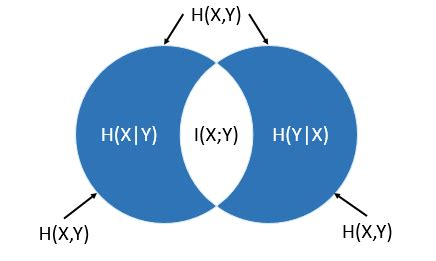
\includegraphics[width=.4\textwidth]{images/MI}\\
\end{center}
\begin{tiny}
Mutual Information: incongruent - congruent stimuli
\end{tiny}
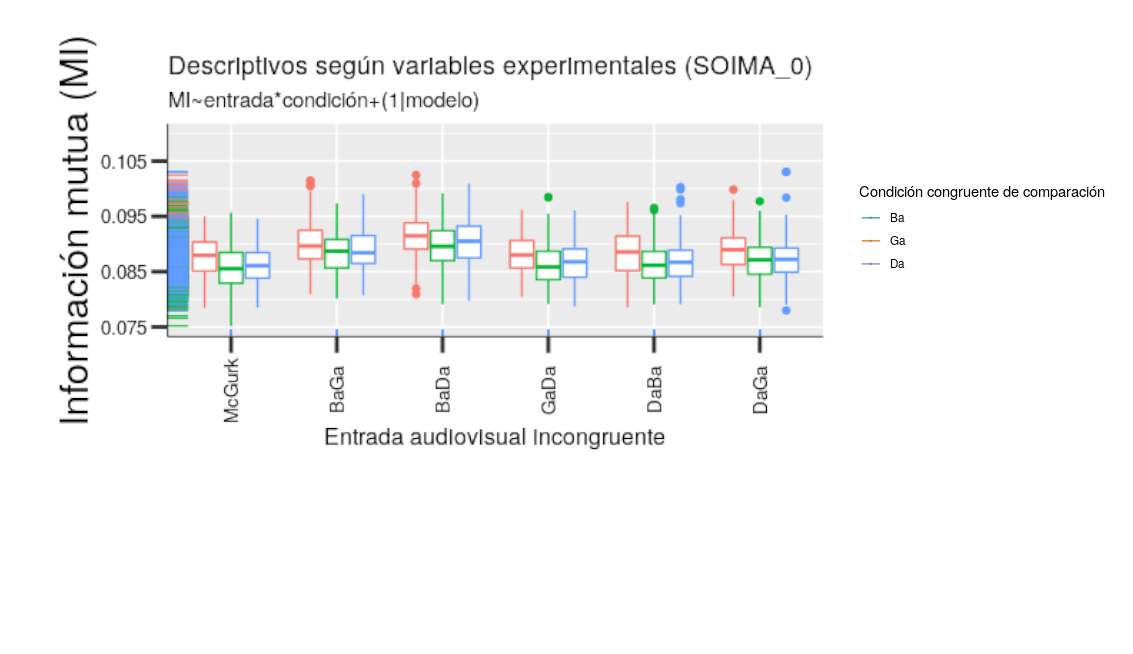
\includegraphics[width=\textwidth]{images/SOIMA0_MI}
\column{.6\textwidth}
\begin{center}
\begin{tiny}
Linear Mixed Effects analysis
\end{tiny}
\end{center}
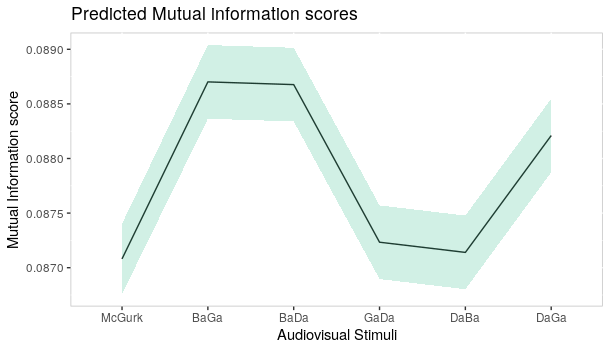
\includegraphics[width=\textwidth]{images/input}
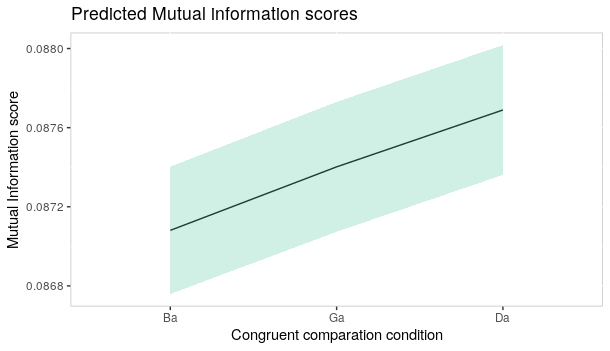
\includegraphics[width=\textwidth]{images/condition}
\end{columns}
\end{frame}



\begin{frame}
\centering

\includegraphics[width=.8\textwidth]{images/thanks}
\end{frame}


\bibliography{library/library}
\bibliographystyle{apalike}

\end{document}
